\section{瓶颈与动机}
\label{sec:motivations}

我们观察到，智能体推理任务中存在严重的 GPU 利用不足。
进一步分析表明，由于每个节点上单个存储 NIC 的带宽有限，KV-Cache 加载速度成为瓶颈。
如下所述，三个决定性因素共同导致了这一瓶颈。


第一，智能体工作负载具有很高的 KV-Cache 命中率，这意味着它们\emph{需要更多 I/O、更少计算}，从而形成严重 I/O 瓶颈。
智能体工作负载天然具有长上下文、短追加和多轮交互特征。
在每一轮中，GPU 需要从持久化存储读取整个上下文的 KV-Cache，并对追加 token 执行 prefill 计算。
我们从代表性代码任务中收集的 trace 显示，平均轮数为 157，说明 LLM 倾向于进行多轮交互。平均上下文长度为 32.7k，而平均追加长度只有 429，这对应 98.7\% 的 KV-Cache 命中率。
在这种场景下，cache-compute ratio，即需要加载的 KV-Cache 与所需计算量的比值，对于 DeepSeek-V3.2~\cite{DeepSeekV32} 约为 22 GB/PFLOP，对存储带宽构成显著瓶颈。
需要注意的是，DeepSeek MLA 模型的 KV-Cache 大小已经高度优化；对于 KV-Cache 更大的模型（见 \autoref{tab:cache-compute-ratio}），情况会更糟。
DeepSeek-V3.2 的比值高于 DeepSeek-V3~\cite{deepseekv3}，这是因为它的稀疏 attention 设计降低了计算需求。

\begin{table}[t]
  \centering
  \caption{\normalfont 追加长度为 429 时，不同上下文长度（16k--64k）下的 cache-compute ratio。除非特别说明，KV-Cache 数据类型默认使用 FP8。}
  \begin{tabular}{lc}
  \toprule
  Model & GB/PFLOP (16K--64K) \\
  \midrule
  % Gemma3-27B~\cite{gemmateam2025gemma3technicalreport} (FP16) & 1.0 \\
  Qwen2.5-32B~\cite{qwen2025qwen25technicalreport} (FP16) & 117-267 \\
  % DeepSeek-V3.2 27B~\cite{DeepSeekV32} & 70--184 \\
  GPT-OSS-120B~\cite{GPT-OSS} & 47--95 \\
  Qwen3-235B-A22B~\cite{yang2025qwen3technicalreport} & 39--60 \\
  DeepSeek-V3.2 660B~\cite{DeepSeekV32} & 13--36 \\
  % Kimi-K2-Base 1T~\cite{kimiteam2026kimik2openagentic} & 0.028 \\
  DeepSeek-V3 660B~\cite{deepseekv3} & 4.8--5.8 \\
  \bottomrule
  \end{tabular}
  \label{tab:cache-compute-ratio}
\end{table}

第二，\emph{硬件演进趋势}并不适合智能体推理工作负载。
近年来，网络带宽和 HBM 容量的增长落后于 GPU FLOPS 的增长，这使智能体工作负载更容易撞上内存墙和通信墙。
如 \autoref{fig:motivation} 所示，从 NVIDIA Ampere 到 Blackwell，I/O-compute ratio 下降了 14.4$\times$。
较低的 NIC 带宽限制了 KV-Cache 加载速度，使 GPU 处于空闲状态。
此外，较小的 HBM 容量限制了 GPU kernel~\cite{ICLR24:FlashAttention2, FlashInfer, DeepGEMM, FlashMLA} 可同时计算的 token batch size，阻碍了 Tensor Core 等计算单元的充分利用~\cite{SOSP25:PrefillOnly}。% Small HBM capacity also limits the overlapping between computation and KV-cache transfers, which requires extra buffer, causing transfer latency to fall on the critical path.

第三，现有 LLM 推理系统在不同 engine 类型之间存在严重的\emph{存储网络利用不均衡}。在流行的 PD 解耦系统中，命中 token 的 KV-Cache 只由 prefill engine 直接从远端存储加载。这种设计将全部存储 I/O 压力集中到 prefill 侧 SNIC 上，而 decode engine 上的 SNIC 基本保持空闲。因此，聚合存储网络带宽无法被充分利用。% This static assignment of the KV-Cache loading role creates a fundamental and inefficient imbalance in storage network bandwidth utilization across engine types.

\begin{figure}[t!]
  \centering
  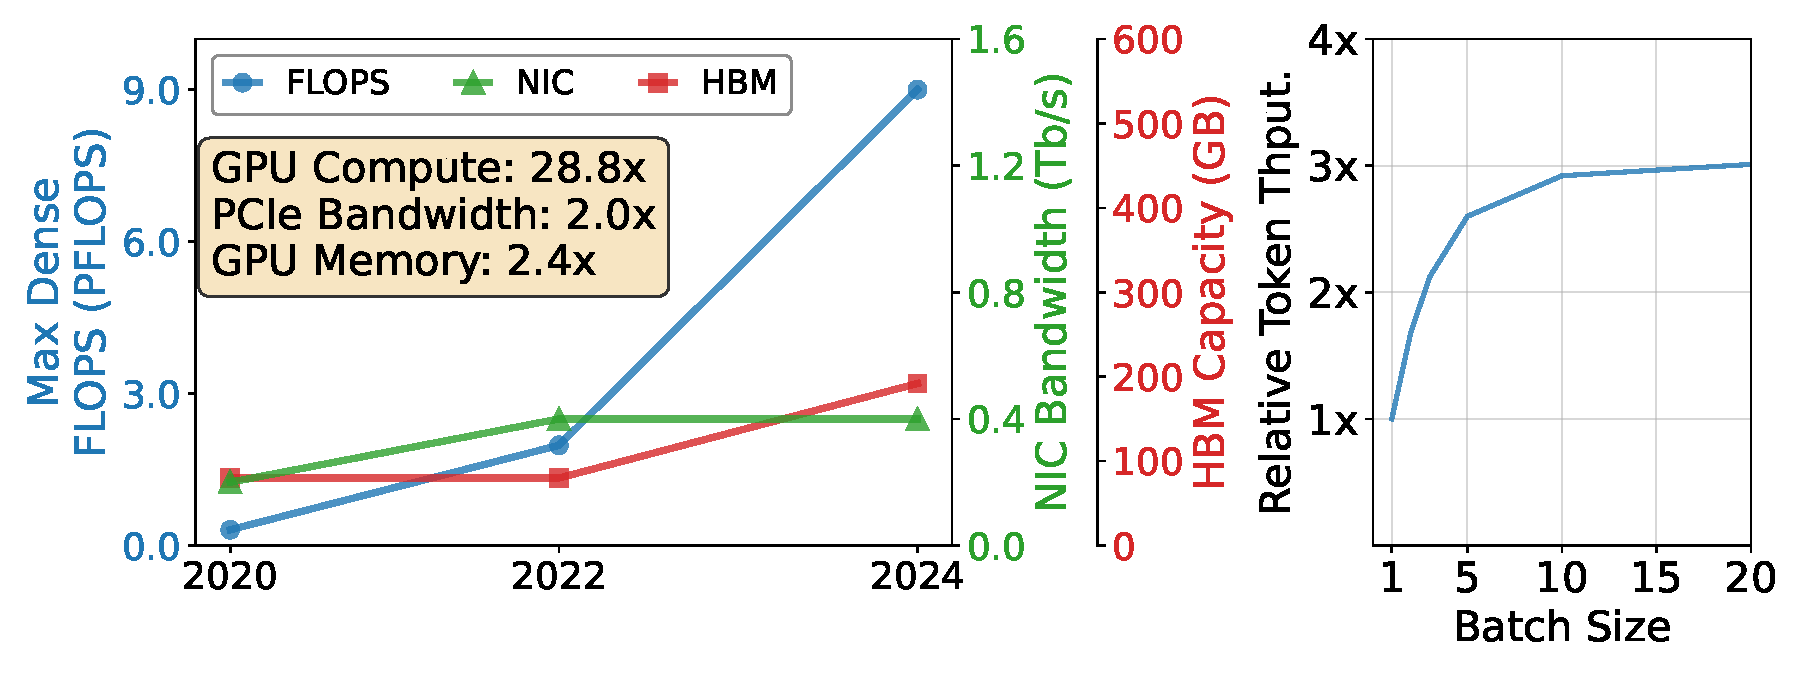
\includegraphics[width=1.05\linewidth]{figures/motivation.pdf}
  \vspace{-0.35in}
  \caption{\normalfont 左：NVIDIA GPU 的硬件趋势。右：不同请求 batch size 下的相对 token 吞吐量（每个请求包含 30K 上下文和 300 个追加 token）。}
  \vspace{-0.2in}
  \label{fig:motivation}
\end{figure}


上述分析表明，在 PD 解耦架构上，智能体推理的根本性能问题是 KV-Cache 取回带来的高 I/O 需求，以及推理 engine 之间存储网络带宽利用不均。同时，我们观察到计算网络的流量具有间歇性模式：模型推理中的 collective 操作以亚毫秒级 burst 形式出现，而计算网络的聚合带宽又远高于存储网络。因此，一个机会自然出现：可以利用 decode 节点的 SNIC 带宽从存储加载 KV-Cache，再利用更快计算网络的空闲带宽将其传回 prefill 节点。
